\documentclass{article}
\usepackage{main}

\title{Translations du plan}
\date{16 Septembre 2024}
\author{Seconde 9}

\begin{document}
\maketitle
\section*{Dérive d'une bouée en mer}
Une bouée destinée à l'évaluation des courant est lâchée en mer le 16 Mai 2024 à 20h. Le repère ci-contre indique la position initiale de la bouée (en $O$), ainsi que sa position le 17 (en $A$), le 18 (en $B$), le 19 (en $C$) et le 20 (en $D$), à la même heure. 
\begin{center}
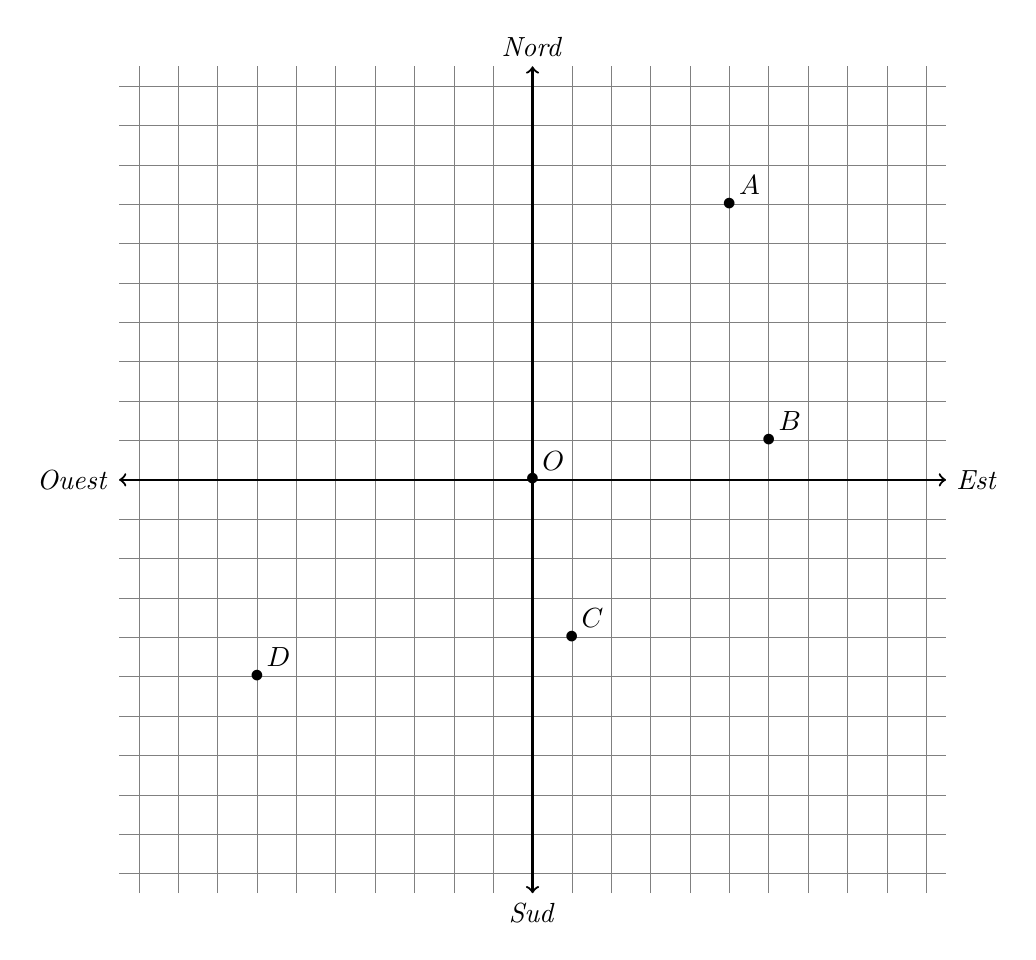
\begin{tikzpicture}
\draw[help lines] (-5.25,-5.25) grid[step=0.5] (5.25,5.25);
\draw[thick,<->] (-5.25,0) node[left] {\emph{Ouest}} -- (5.25,0) node[right] {\emph{Est}}; 
\draw[thick,<->] (0,-5.25) node[below] {\emph{Sud}} -- (0,5.25) node[above] {\emph{Nord}};

\draw (0,0) node {$\bullet$} node[above right] {$O$};
\draw (2.5,3.5) node {$\bullet$} node[above right] {$A$};
\draw (3,0.5) node {$\bullet$} node[above right] {$B$};
\draw (0.5,-2) node {$\bullet$} node[above right] {$C$};
\draw (-3.5,-2.5) node {$\bullet$} node[above right] {$D$};
\end{tikzpicture}
\end{center}
\begin{enumerate}[label=\emph{\alph*)}]
\item En vous inspirant du premier point, compléter les descriptions suivantes:
\begin{enumerate}[label=\arabic*.]
\item Entre le 16 et le 17 Mai, la bouée s'est déplacée de $5$ unités vers l'est, et de $7$ unités vers le Nord.
\item Entre le 17 et le 18 Mai, la bouée s'est déplacée \answersline
\item Entre le 18 et le 19 Mai, la bouée s'est déplacée \answersline
\item Entre le 19 et le 20 Mai, la bouée s'est déplacée \answersline
\end{enumerate}
\item Placer les points $E$, $F$ et $G$ correspondant aux jours suivants d'après les intructions suivantes:
\begin{enumerate}[label=\arabic*.]
\item Du 20 au 21 Mai ($E$) : la bouée s'est déplacée ce jour-là d'$1$ unité vers l'est, et de $5$ vers le nord.
\item Du 21 au 22 Mai ($F$) : la bouée s'est déplacée de la même manière que du 17 au 18 Mai.
\item Du 22 au 23 Mai ($G$) : la bouée a suivi le déplacement opposé que celui du 18 au 19 Mai.
\end{enumerate}
\item Une nouvelle bouée est lachée le 3 Août en $O$. On remarque qu'en un jour, la bouée a parcourru le même déplacement que la première bouée entre le 18 et le 21 Mai. Placer le point $A'$ correspondant à la position de cette nouvelle bouée.
\end{enumerate}
\end{document}